\documentclass[8pt,twocolumn]{article}
\usepackage[utf8]{inputenc}
\usepackage[english,main=italian]{babel} 
\usepackage[margin=0.5in]{geometry}
\usepackage[T1]{fontenc}


\usepackage{url}
\usepackage{hyperref}
%random
\usepackage{verbatim}
\usepackage{xcolor}
\usepackage{amsmath}
\usepackage{amssymb}
\usepackage{mathtools}

\DeclarePairedDelimiter\ceil{\lceil}{\rceil}
\DeclarePairedDelimiter\floor{\lfloor}{\rfloor}

%img
\usepackage{graphicx}
\graphicspath{ {img/} }

%title
\usepackage{listings}
\usepackage{geometry}


%%% customization della testa e del footer
\usepackage{fancyhdr}
\pagestyle{fancy}
\fancyhf{}
\rhead{Luca Vecchi}
\lhead{Visione artificiale 2019}
\lfoot{\date{\today}}
\rfoot{Pag.: \thepage}

%%% inline quote
\usepackage{csquotes}
\DeclareQuoteStyle[american]{english}
    {\itshape\textquotedblleft}
    [\textquotedblleft]
    {\textquotedblright}
    [0.05em]
    {\textquoteleft}
    {\textquoteright}
        
\setlength\columnsep{3em}

\selectlanguage{italian}

%samepage no pagebreake after section
%\usepackage{samepage}
\begin{document}
    \title{Progetto Visione Artificiale 2019\\\\
        Hough Voting F-Formation \& Graph Cut for F-Formation\\
        \medium Esposizione, Implementazione, Valutazione}
    \author{Luca Vecchi}
    \date{\today}
    \maketitle
    \begin{abstract}
    	Nell'ambito della computer vision il riconoscimento automatico del comportamento sociale dei gruppi è un importante task, utile nei campi della video sorveglianza, robotica sociale e dell'interazione umana. Nel seguente elaborato verranno trattate due metodologie per il riconoscimento di gruppi o meglio \textit{Free-standing Conversation Group} (FCG) in cui i soggetti sono impegnati in un'interazione reciproca, comune, focalizzata ed esclusiva che porta i partecipanti a creare disposizioni nello spazio denominate \textit{Facing Formation} o \textit{F-formation}. I metodi di \textit{Hough voting F-formation}\cite{Cristani:BMVC11} e \textit{Graph Cut F-formation}\cite{Setti:PLOS15} si pongono l'obiettivo utilizzando unicamente segnali sociali visivi, sotto le ipotesi di camera calibrata e possibilità di stimare la posizione e l'orientamento della persona, di ricavare la sotto struttura \textit{o-space} dell'F-formation condizione necessaria per la presenza di un FCG. Nel primo caso si propone un algoritmo basato su una strategia di voti in un particolare spazio di Hough mentre nel secondo un procedimento iterativo basato su tagli di grafi e aggiornamenti di pesi.\\
    	Sono esposti dapprima la terminologia, i concetti base e le ipotesi in cui si pongono i due metodi. Si espongono i dataset e il setup sperimentale usati per la valutazione delle prestazioni.
    	Successivamente saranno trattati i due algoritmi esibendo lo pseudocodice, eventuali parametri per concludere con risultati e confronti tra i due metodi trattati.
    \end{abstract}

	
	\section{Introduzione}
	
	%ragione del problema
	
	%definizioni varie:
	% [x] gruppi
	% [x] interazioni sociali
	% [x] FCG
	% [x] f-formation
	% [x] t-segment
	Con interazioni sociali intendiamo \enquote{i comportamenti, azioni di due o più persone orientate in modo reciproco verso loro stessi; comportamenti che coinvolgono e provocano nell'altro soggetto un'esperienza}. I gruppi invece sono aggregazioni composte da individui in cui si svolgono dal punto di vista sociale azioni e interazioni reciproche. Questa prima definizione viene ripresa dallo stesso Cristiani et Al.\cite{Cristani:BMVC11} e ridefinendo e specificando ulteriormente la struttura sociale sotto indagine. Esso indica il voler analizzare l'interazione tra \textit{assemble/gruppi} \footnote{Indica in modo specifico la differenza tra il termine \textit{group} e \textit{gathering}.	Il primo indica una relazione duratura di appartenenza e di organizzazione, il secondo esalta la facilità e la limitatezza nel tempo.} formato da persone \textit{congiuntamente focalizzate} nell'interazione in modo \textit{quasi statico} in una scena dinamica. Con congiuntamente focalizzate nell'interazione indichiamo quei individui che accettano, per tacito consenso o non, di mantenere per un periodo di tempo un attenzione cognitiva tra loro; trattiamo della differenza tra l'interazione di soggetti riuniti in una riunione piuttosto di individui in attesa o che collettivamente guardano un film. Con interazione semi-statica piuttosto che dinamica indichiamo la durata del'interazione che, per fare un esempio, può includere nel primo caso una partita di scacchi e nel secondo caso interazioni veloci come quella durante un ordinazione al ristorante.\\
	
	I \textbf{Free-standing conversation group} (\textbf{FCG}) fanno parte della classe di aggregazioni sociali sopra indicata ma restringono il campo a quelle interazioni in cui gli individui interagiscono in piedi. E' il caso delle persone che conversano davanti una \textcolor{red}{vending-machine}. Nei FCG le persone interagiscono ed esibiscono determinate azioni non verbali dette \textit{social signal} che si possono osservare sotto forma di posizioni e orientazioni rispetto al gruppo: i \textbf{Facing Formation}.
	
	Il termine coniato da Adam Kendon\cite{kendon1990conducting}, F-formation, come lui indica:
	\begin{quote}
	    An F-formation arises whenever two or more people sustain a spatial and orientational relationship in which the space between them is one to which they have equal, direct, and exclusive access.
	\end{quote}
	
	\begin{figure}
	    \centering
	    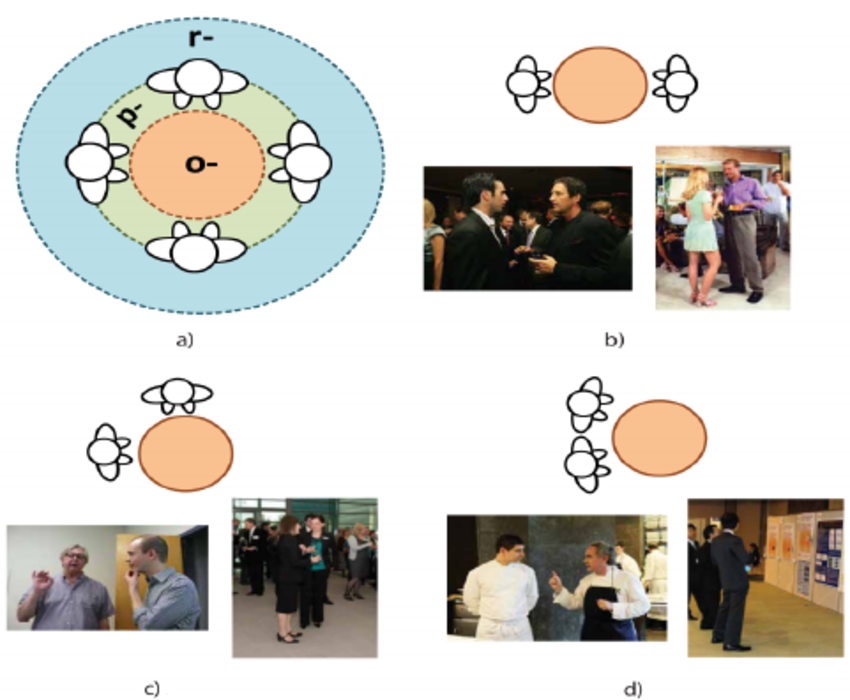
\includegraphics[width=0.8\linewidth]{f_formation}
	    \caption{Esempi di F-formation}
	    \label{fig:f_formation}
	\end{figure}
	
	Una F-formation, come si può vedere in figura \ref{fig:f_formation} è una partizione dello spazio in tre spazi sociali:
	\begin{description}
    	\item [p-space] è la partizione dello spazio che racchiude l'\textit{o-space} e che contiene le persone che partecipano all'interazione
    	\item [o-space] spazio convesso, vuoto, circondato dal \textit{p-space} e usato dalle persone per interagire. Esso può essere definito come l'intersezione dei \textbf{transactional segment}(t-segment) delle persone nel \textit{p-space} che non sono altro che la sovrapposizione del campo di visione e attenzione cognitiva
    	\item [r-space] è la zona intorno al \textit{p-space} che include le altre due aree
	\end{description}
	
	Nonostante l'r-space sia importante tanto quanto l'o-space per via che può definire persone ignorate, fasi di inserimento/uscita dall'o-space, in entrambi gli algoritmi si cerca di stimare l'o-space e i partecipanti del p-space.
	
	Come si può osservare in figura \ref{fig:f_formation} ci possono essere varie disposizioni spaziali-orientazioni dei soggetti nella F-formation che danno luogo a diverse disposizioni, in ordine: disposizione \textit{vis-a-vis} , disposizione ad \textit{L} e disposizione \textit{side-by-side}. Oltre a questa anche altre (ferro di cavallo, rettangolare, lineare, ecc.).
	
	
	\subsection{Dataset}
	I dataset \footnote{\url{http://profs.scienze.univr.it/cristanm/ssp/download/data.zip}} sono organizzati nel seguente modo:
	\begin{description}
	    \item [features]: contiene per ogni frame $<ID,x,y,\alpha>$ dove $ID$ è il nome univoco, $(x,y)$ è la proiezione sul terreno delle posizioni dei soggetti e $\alpha$ è l'orientamento del \textit{t-segment}
	    \item [groundtruth]: contiene per ogni frame $G_{i,...,j}^1,...,G_{q,...,k}^M$, $M$ F-formation, ognuna contenente gli ID che partecipano all'interazione (per gruppo $G^1$ $i,j \in G^1$)
	    \item [settings]: contiene per il dataset la definizione di due parametri quali il raggio del'o-space o \textit{stride} e il \textit{minimum description lenght}  (MDL)
	    \item [settings\_gc]: contiene un vettore con gli elementi in ordine: raggio, matrice di covarianza, empty, nsamples, quant, s. I parametri fondamentali sono la matrice di covarianza per effettuare il campionamento (multivariato nella posizione x-y e nell'orientamento), il numero di campionamentit da effettuare e il valore di un singolo quanto\footnote{TODO guardare differenza tra raggio e stride perchè dovrebbero essere la stessa cosa ma uno è il doppio dell'altro}.
	\end{description}
	\begin{description}
	\item [Synthetic]: 
	\item [IDIAP Poster]:
	\item [Cocktail Party]:
	\item [Coffe Break]:
	\item [GDet]:
	\end{description}
	
	
	%introduzione approci
	%aspetti innovativi
	%setup sperimentale
	%dataset
	%\input{chapter/intro}
	\section{Metodologie}
	\subsection{HVFF}
    \subsubsection{Algoritmo}
	\subsubsection{Parametri}
	\subsection{GCFF}
    \subsubsection{Algoritmo}
	\subsubsection{Parametri}
	\section{Risultati}
	\subsection{Analisi efficacia}
	\subsection{Conclusioni}
	
	
	
	\newpage
	\onecolumn
	\bibliographystyle{unsrt}
	\bibliography{bib}
\end{document}
